\documentclass[12pt]{article}
\sloppy %prevent text overflowing margins

\usepackage{amsmath}
\usepackage{graphicx}
\usepackage{mathtools}
\usepackage{subcaption}
\usepackage{float}
\usepackage[none]{hyphenat} %prevent hypenation
\usepackage[margin=2.5cm]{geometry}\usepackage[square]{natbib}
\usepackage{setspace}
\onehalfspacing %sets line spacing to 1.5

\usepackage{xcolor,colortbl}

\definecolor{myyellow}{RGB}{247, 230, 96}
\definecolor{myblue}{RGB}{162, 197, 242}
\definecolor{mygrey}{RGB}{214, 214, 214}

\title{Practical Data Compression - Project Plan}
\author{\textbf{Lewis Wilson} \\
	BSc Mathematics with Computer Science\\\\
	Department of Mathematics, College of Engineering,\\ 
	Design and Physical Sciences, Brunel University.\\\\
	Supervisor: Aleksey Pichugin}
\date{Year of Submission: 2017/2018}
\begin{document}
	\begin{titlepage}
	\maketitle
	\thispagestyle{empty} %Removes page number
	\end{titlepage}
	
	\setcounter{page}{1} %begin from page 1 here
	
	
	\section{Data Compression}
	\subsection{Prerequisites}
	To become familiar with practical data compression, it is essential to have:
	
	\begin{itemize}
		\item A good understanding of computer data structures, hexadecimal counting systems and how binary operations are performed;
		\item Knowledge on how algorithms function and how computers interpret these algorithms;
		\item An idea of how digital storage and efficiency is calculated;
		\item An understanding of mathematical fundamentals including sets, matrix computation, simple trigonometry and basic probability theory \citep{ipu_dc}.
	\end{itemize}

	\begin{flushleft}
		Supplementary to these prerequisites, it would be helpful to have the following skills:
	\end{flushleft}
	
	\begin{itemize}
		\item A knowledge of encoding schemes such as the American Standard Code for Information Interchange (ASCII) and Unicode, to be able to understand how bytes are converted into characters;
		\item An understanding of a programming language, preferably Matlab/Octave, as implementations will be written as such.
	\end{itemize}
	
	\subsection{Background}
	Compression has become essential in the age of computers, as data is constantly created and rarely deleted. With this trend in data creation, both the requirements for storage capacity increase and efficiency in data compression have become important.
	
	General computer users are often subject to data compression, with `Zipped' (ZIP) and Roshal Archive (RAR) files commonly acting as compressed containers to store many/large data items in. Behind compressed file types are specific methods to achieving their compression, some of which are to be discussed in this paper.
	
	As well as saving storage space for users locally on their hard-drives, compression has become important since the birth of the public  internet. Many services on the internet enable users to access large amounts of data in a short period of time. One such example of these services is Netflix for streaming audio and video data. Without data compression applied, streaming services would be far less efficient both for hosts and clients; raw video consumes a vast amount of bandwidth, therefore using compression helps to achieve transmission efficiency \citep{internet_video_streaming}. 
	
	There are two types of data compression, lossless and lossy. Lossless compression reduces the size of data without the loss of content after decompression, whereas lossy compression conversely removes any seemingly unnecessary articles from the data, thus reducing its size.
	
	There are many different algorithmic approaches to compression. These methodologies include: statistical, dictionary based and wavelet based approaches. As examples, Huffman Coding provides a statistical method of approach, whereas Lempel-Ziv-77 (LZ77) is dictionary based \citep{dc_complete_ref}. It is not uncommon for a combination of approaches to be applied. Taking DEFLATE as an example algorithm, this uses a combination of LZ77 and Huffman Coding to achieve compression.
	
	One issue in the domain of compression are the speeds of compressing and decompressing data. Often there is a trade-off between amount of compression and speed of compressing/decompressing the data \citep[p.~5]{dc_complete_ref}. 
	
	
	\subsection{Motivation}
	Having had an interest in computers for a number of years and studying Mathematics with Computer Science, I was drawn to a project involving a combination of both subjects. During my placement year, I had a conversation with a colleague about data compression and the underlying technologies. Since then, I have been fascinated by the idea of storing large amounts of data in smaller spaces, whilst maintaining the full data set (lossless compression).
	
	To supplement my learning, I have also chosen to take the Mathematics module MA3236: Data Compression and Encryption. While encryption can be applied during compression of data, it is out of scope for this project.
	
	\subsection{Applications}
	There are many lossless compression algorithms that have practical implementations. Some such example algorithms include \citep[p.~1050-1065]{dc_complete_ref}:
	
	\begin{itemize}
		\item \textbf{Huffman Coding}: a method of lossless compression used in a variety of popular computer programs;
		
		\item \textbf{LZ77}: a dictionary based method used as the basis of all dictionary compression methods. LZ77 and its variants are used in reducing text, image and audio file sizes;
		
		\item \textbf{RAR}: Popular with Windows users, has options for error-correcting and encrypting stored data. RAR was initially a variant of LZ77, however has been thoroughly developed since its initial release;
		
		\item \textbf{Free Lossless Audio Compression (FLAC)}: used to compress audio files while maintaining their quality.

	\end{itemize}
	
	\section{Huffman Coding}
	Huffman Coding, developed by David Huffman in 1952, is a popular lossless method of compressing data often used in combination with other techniques for enhanced compression \citep{dc_complete_ref}. The encoding process, takes each symbol (or character) of a message and represents it with a binary value of varying length.
	
	An important aspect of Huffman Coding, is its attention to symbol frequencies within a set of raw data. The underlying concept of Huffman is to allocate a smaller number of bits (0s and 1s) to the symbols with a higher rate of occurrence. For example, in the string,	\textbf{aaaabcd}, the symbol \textbf{a} is likely to have an encoded value of a single 1 or 0, whereas \textbf{b}, \textbf{c} and \textbf{d} will probably have values exceeding 1-bit in length (e.g. 01 or 010).
	
	\subsection{Example}
	This section will describe how to encode a piece of data using Huffman Coding.
	
	\begin{itemize}
		\item Take a piece of data, say the string: \textbf{aabbbccccd};
		
		\item The frequency of each symbol can be represented in matrix form as,		
		$\begin{pmatrix}
			a & 2 \\
			b & 3 \\
			c & 4 \\
			d & 1
		\end{pmatrix}$
	\end{itemize}
	\begin{itemize}
		\item Combining the symbols in the matrix with the lowest frequency values, and iterating until one entry is left, we get:
	\end{itemize}
	\begin{equation*}
		\begin{pmatrix}
		a & 2 \\
		b & 3 \\
		c & 4 \\
		d & 1
		\end{pmatrix}
		\rightarrow
		\begin{pmatrix}
		ad & 3 \\
		b & 3 \\
		c & 4 
		\end{pmatrix}
		\rightarrow
		\begin{pmatrix}
		adb & 6 \\
		c & 4 
		\end{pmatrix}
		\rightarrow
		\begin{pmatrix}
		adbc & 10
		\end{pmatrix}
	\end{equation*}
	\begin{itemize}
		\item Working backwards through the iterative process, we can generate a tree structure, known as a Huffman Tree (Figure \ref{fig:huff_no_bin}). This tree shows how concatenations of symbols were created.
	\end{itemize}
	\begin{figure}[H]
		\centering
		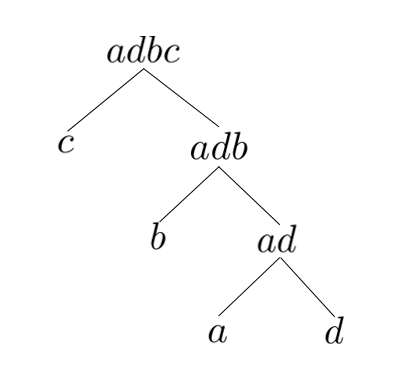
\includegraphics[scale=0.6]{../Images/Huffman_tree_no_binary.png}
		\caption{Huffman Tree without Binary Representation}
		\label{fig:huff_no_bin}
	\end{figure}
	\begin{itemize}
		\item Appending each left path with a 1 and each right path with a 0, we generate a Huffman Tree with binary symbol representations (Figure \ref{fig:huff_with_bin}). Traversing the tree from the root node, the binary representations can then be allocated to the symbols.
	\end{itemize}
	
	\begin{figure}[H]
		\centering
		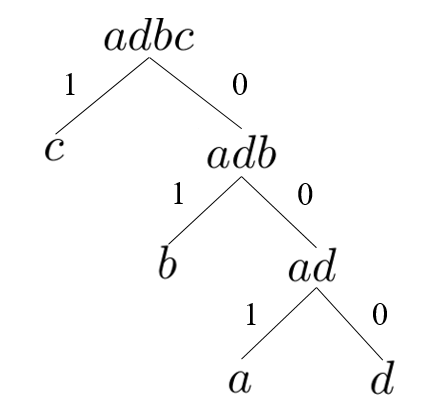
\includegraphics[scale=0.5]{../Images/Huffman_tree_with_binary.png}
		\caption{Huffman Tree with Binary Representation}
		\label{fig:huff_with_bin}
	\end{figure}

	Here, the binary representations are: \textbf{a = 001, b = 01, c = 1 and d = 000}. So the final encoded string is: \textbf{0010010101011111000}.
	
	Assuming each symbol in the un-encoded data has a length of 8-bits (1-byte), the un-encoded data has a total size of $10\cdot8 \text{-bits} = 80\text{-bits}$. The encoded data has a size of $19\text{-bits}$. Therefore providing a compression rate of $(19\div80)\cdot100 = 23.75\%$.
	
	\section{LZ77}

	Lempel-Ziv-77 is a lossless algorithm used for data compression. It was produced by Jacob Ziv and Abraham Lempel in 1977 \citep{lz77}. The paper written in 1977 provides an idea to compress data using a `search buffer' and a `look-ahead window', whereby the look-ahead window characters are read in order; the algorithm searches for a match for the current look-ahead window character in the search buffer. If the character is found, the next value in the look-ahead window is appended, and again the search buffer is checked, to see if a previous match already exists.
	
	Although the paper \citep{lz77} provides a large amount of theory, it gives little information on how to encode and decode the data. To apply encoding with LZ77, I shall focus on one particular LZ77 variant, LZ4.
	
	\subsection{Example}
	This section provides a short example of LZ77. Assume that the data on the left of the vertical bar has been encoded and is part of the search buffer, and that the data on the right is yet to be encoded and is part of the look-ahead buffer. \emph{Note: offset is denoted as the number of characters to traverse backwards in the search buffer from right to left}.
	
	\begin{equation*}
		\textbf{abccbccbba\textbar bccbcc}
	\end{equation*}
	
	The LZ77 encoder reads the first character from the look-ahead buffer, `\textbf{b}'. The search buffer is then traversed from right to left looking for a match. At offset `2', a match is found. Appending the next character to gain the string `\textbf{bc}', the search buffer is checked to see if the match at offset `2' contains \textbf{bc}, it does not. The search buffer is checked for any other matches that correspond to `\textbf{bc}', one of which is found at offset `6'. Again the next look-ahead buffer character is appended, `\textbf{bcc}'. This process continues until no more matches can be determined in the search buffer. Tokens are created to determine references to the search buffer during decoding of the data. The process repeats iteratively.
	
	\section{LZ4}

	Lempel-Ziv-4 is a modern algorithm, based on the popular LZ77 method. It is currently Open-Source Software (OSS), used by Operating Systems (OS), file systems, games, storage systems, databases and other technologies and is avaliable at \citep{lz4_github}. The algorithm works using sequences/blocks. Figure \ref{fig:lz4_ss} shows the standard block format.
	
	\begin{figure}[H]
		\centering
		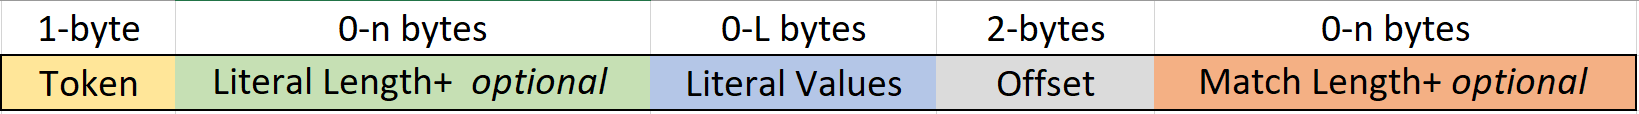
\includegraphics[scale=0.45]{../Images/LZ4_Sequence_Structure.png}
		\caption{LZ4 Sequence Structure}
		\label{fig:lz4_ss}
	\end{figure}
	
	In Figure \ref{fig:lz4_ss}, each section is defined as follows \citep{how_lz4_works}, \citep{lz4_explained}:
	
	\begin{itemize}
		\item \textbf{Token}: a 1-byte field, where the upper 4-bits relate to the number of literals and the lower 4-bits relate to the length of the data match found;
		
		\item \textbf{Literal Length+}: Extra allocated space in the event that the number of literals exceeds the maximum of 15 (1111) in the token;
		
		\item \textbf{Literal Values}: The character/symbol values;
		
		\item \textbf{Offset}: How many characters to traverse in the current string from the tail end; 
		
		\item \textbf{Match Length+}: Extra allocated space in the event that the length of the data match exceeds the maximum of 15 in the token (1111).
	\end{itemize}
	
	\subsection{Example}
	For clarity, I will provide a worked example of LZ4 on sample data. An example of encoded LZ4 data (matched with the format in Figure \ref{fig:lz4_ss}) could be given as:
	
	\begin{center}
		\setlength{\tabcolsep}{1pt}
		\begin{tabular}{c c c c c c c c c c c}
			\textbf{\#} & \textbf{\cellcolor{myyellow}{40}} & \textbf{\cellcolor{myblue}{abcc}} & \textbf{\cellcolor{mygrey}{+3}} & \textbf{\#} & \textbf{\cellcolor{myyellow}{13}} & \textbf{\cellcolor{myblue}{b}} & \textbf{\cellcolor{mygrey}{+9}} & \textbf{\#} & \textbf{\cellcolor{myyellow}{00}} & \textbf{\cellcolor{mygrey}{+0}}
		\end{tabular}
	\end{center}
	
	\emph{Note: Each numeric value is written here in hexadecimal, while ``\#" represents the beginning of a token.}
	
	The iterative process to decode the data is as follows:
	
	\begin{itemize}
		\item After the first token, copy the literals written (the length of literals being the higher 4-bits within the token, `4' in our case): \textbf{abcc}
		
		\item Read the offset value (+3 for us) and traverse the current string backwards on a per character basis. Here I will use `\textbf{!}' to denote the current position: \textbf{a!bcc}
		
		\item Temporarily focus on the current position marker to the end of the current string. In our case the string: \textbf{bcc}. This string will be called our `temporary string'.
		
		\item Using the final 4 bits of the token plus 4 (as LZ4 defines a minimum match length of 4), copy this number of characters from the temporary string. (For us, $0+4=4$) \emph{If the number is larger than the length of the temporary string, then once the maximum value is reached, start again from the beginning of the temporary string}: abcc\textbf{bccb}
		
		\item Iterate this process until the token \textbf{\#00+0} (ending token) is reached.
	\end{itemize}

	After the second (and final) iteration, our decoded data becomes:
	
	\begin{equation*}
		\textbf{abccbccbbabccbcc}
	\end{equation*}

	\clearpage
	\section{Project Plan}
	\subsection{Overview}	
	Throughout the year, I will be producing functions written in Octave to replicate the types of compression performed by well-known compression methodologies.  I have chosen Octave as it is primarily designed as a mathematical programming application; this feeds nicely into data compression. As well as producing my own code for these techniques, I will also be researching other various approaches in detail. Two specific algorithms intended to be researched further are Huffman Coding and LZ4 (a LZ77 variant).
	
	My main objective is to produce my own versions of Huffman Coding and LZ4 compression, which take input files and compress them accordingly. I am expecting to be able to achieve approximately 70\% compression in each case. Each script I write will display the input and output sizes of the respective files (likely in bits) and will calculate the relative compression based on these values.
	
	As an ambitious aim, dependent on time and progress, I will attempt to write a script incorporating LZ4 compression with a layer of Huffman Coding applied over the LZ4 encoded data - this means that a statistical method will be applied over dictionary encoded data.
	
	\subsection{Objectives}
	I have identified four main objectives to align to this project, these are:
	
	\begin{enumerate}
		\item \textbf{Produce two working data compressors}: At minimum, two data compression algorithms will be implemented, one statistical and one dictionary based;
		
		\item \textbf{Achieve a good level of compression}: Each algorithm produced should achieve a good level of compression. I have estimated that the maximum compression will be approximately 70\% of the size of the original file;
		
		\item \textbf{Understand the suitability of algorithm types}: Become aware of the advantages and disadvantages of different types of algorithm. E.g. Are there certain types of data in which statistical methods are desired over dictionary methods?;
		
		\item \textbf{Deliver a high-quality, detailed dissertation write-up}: This should include how the research is useful and how it aligns to practical scenarios, why the implemented methods were chosen, walkthrough examples of each method performed, advantages and disadvantages and a detailed description of how the work was performed and analysed.
	\end{enumerate}
	
	\subsection{Work Plan}
	The steps for completion of this dissertation project are as follows. Note that the objective that each step aligns to is written in parentheses:
	
	\begin{enumerate}
		\item \textbf{Background Research} \emph{(Obj.3)}: Become familiar with technical terms used in compression and understand the basis of common compression methods and their applications;
		
		\item \textbf{Huffman Coding Research} \emph{(Obj.3)}: Research the fundamentals of Huffman Coding, understand how this method manages to compress data and where it is useful;
		
		\item \textbf{Huffman Coding Implementation} \emph{(Obj.1,2)}: Produce scripts to replicate Huffman Coding (both encoding and decoding). The scripts produced should display the efficiency of the algorithm for numerous types of files;
		
		\item \textbf{LZ4 Compression Research} \emph{(Obj.3)}: Understand how LZ4 is successful in compressing data. Are there types of data that LZ4 will not be efficient in compressing? Understand the advantages and disadvantages of LZ4 against Huffman Coding and other algorithms;
		
		\item \textbf{LZ4 Compression Implementation}\emph{(Obj.1,2)}: Produce a working example of an LZ4 compressor that is able to compress many types of file, with a good compression ratio, and is able to decompress them effectively;
		
		\item \textbf{Huffman Coding with LZ4} \emph{{(Ambitious Goal) (Obj.1,2,3)}}: If I have the time, I will attempt a merging of Huffman Coding with LZ4 compression. This will display the effectiveness of compression algorithm layering;
		
		\item \textbf{Algorithm Analysis} \emph{(Obj.3)}: The scripts I have produced should be further analysed for practical use. Some metrics measured may be the time taken to compress/decompress data and the compression ratio achieved on various types of file;
		
		\item \textbf{Final Write-Up} \emph{(Obj.4)}: My findings should be formally written as per the dissertation guidelines set by the University. The content will discuss each algorithm and my implementation, along with their advantages and disadvantages against each other and industry standard compressors.
	\end{enumerate}

	So far I have successfully created a working Huffman encoder that calculates the compression percentages of input files against their respective encoded format. I am currently in the process of developing a decoder that takes those encoded files and reverts them back to their original state.
	
	\subsection{Gantt Chart}
	
	\begin{figure}[H]
		\centering
		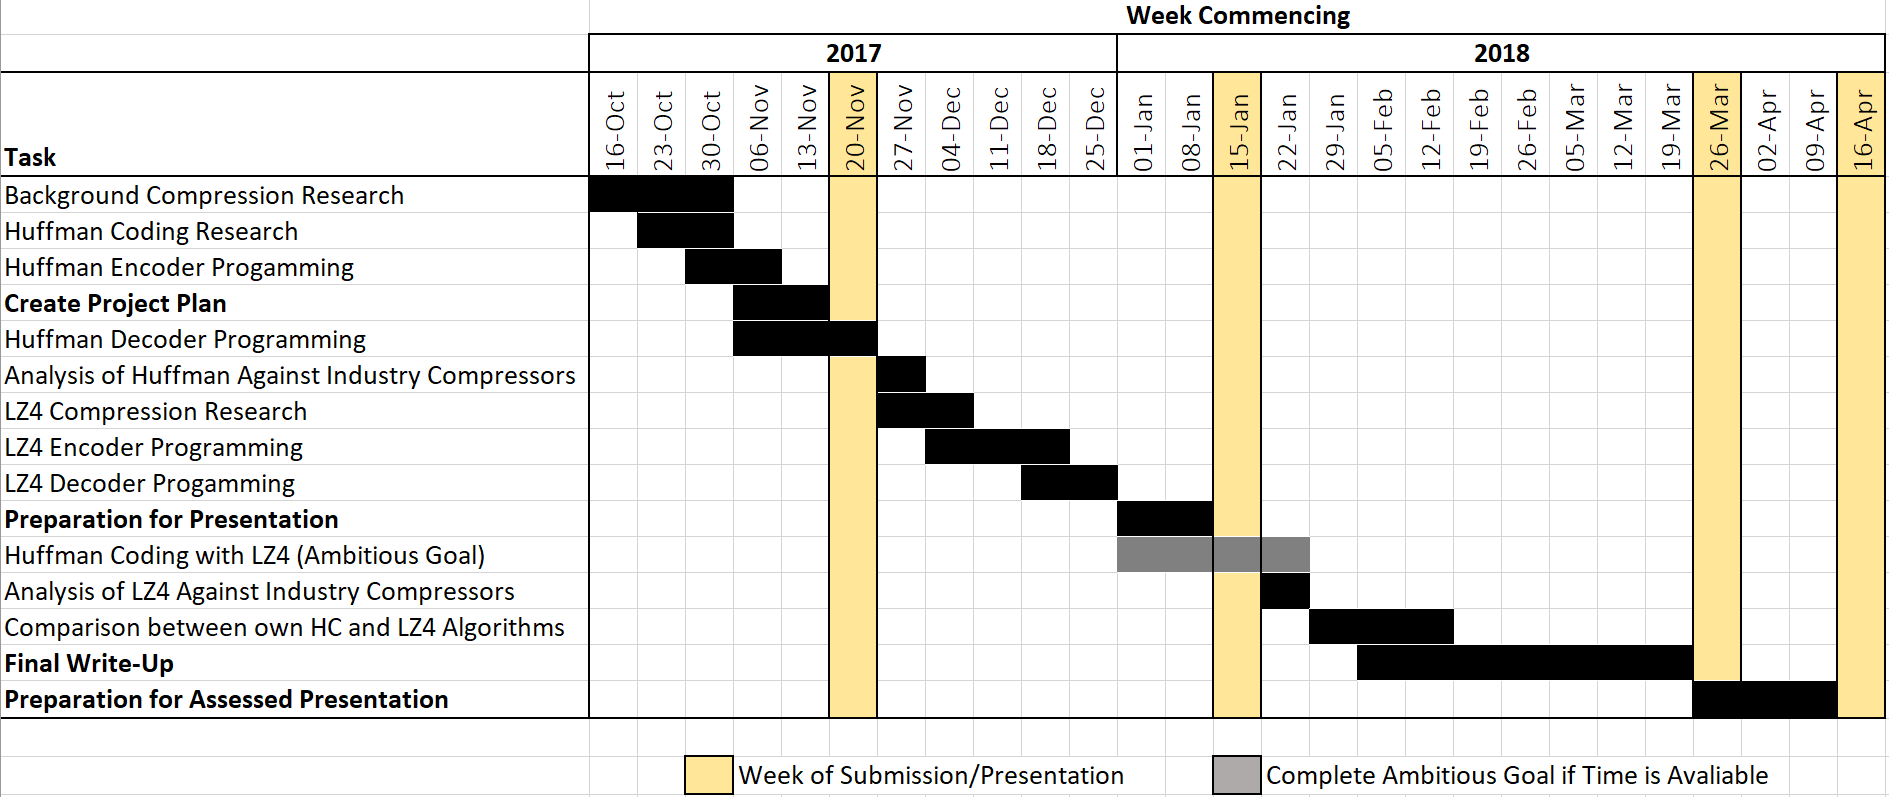
\includegraphics[angle=270, scale=0.5]{../Images/Dissertation_Gantt_Chart.png}
		\caption{Dissertation Gantt Chart}
		\label{fig:gantt_chart}
	\end{figure}

\clearpage
\bibliographystyle{agsm}
\bibliography{../references}
\end{document}

